\documentclass[journal,twoside]{IEEEtran}
\usepackage[pdftex]{graphicx}
\graphicspath{{./gauss/}}
\DeclareGraphicsExtensions{.pdf,.jpeg,.png}
\usepackage{amsmath}
\usepackage{url}
\begin{document}

    \setcounter{page}{55}
\title{A Solution to Gauss Circle Problem}


\author{\IEEEauthorblockN{Hemanta Kunwar}\\
\IEEEauthorblockA{Department of Electrical Engineering\\
Institute Of Engineering(IOE)\\
Pulchowk Campus\\
Pulchowk, Kathmandu\\
Email: \url{maths.std.hkunwar@gmail.com}}
}
\markboth{Zerone Scholar,~Vol.~1, No.~1, November~2016}%
{\textit{H. Kunwar}: A Soltion to Gauss Circle Problem}
\maketitle


\begin{abstract}
In this article, a method of finding number of lattice points within a real-circle having center at origin has been mentioned, which in-fact is the requirement of Gauss Circle Problem. The method involves a simple concept of analytical geometry, basic algebra and number theory.
\end{abstract}




\section{Introduction}
\IEEEPARstart{T}{he} problem was proposed by one of the great mathematician Carl Friedrich Gauss. Simply stated, the problem is all about counting number of points with integer coordinates which are inside a circle of given radius centered at the origin. The solution to this problem was mentioned in Hilbert and Cohn-Vossen 1999.[1] In this article the alternative way to attain same result is mentioned.
 \subsection{Lattice point in $R^{2}$}
A point $(x,y)$ in $R^{2}$ is said to be a lattice point if $x \in Z$ and $y \in Z$.




\section{Problem Statement}
Consider a circle in $\textbf{R}^{2}$ with equation $x^{2}+y^{2}=a^{2}$, $a \geq 0$, how many ordered pairs $(m,n)$ exist, such that $m,n \in Z$ and $m^{2}+n^{2} \leq a^{2}?$ [2]
\section{Solution}
We divide the problem into two cases and provide a solution for both.
\subsection{Case 1: $a \in Z$}
First we consider the line $y=a$ as a reference line. The only reason behind this assumption is that it is used as the reference to count the lattice points. The lines horizontal to $x$-axis, $y=a-1, y=a-2,....,y=0$ are defined as the $1^{st}, 2^{nd},....., a^{th}$ integral line respectively. Clearly, the shortest distance between $k^{th}$ integral line and reference line is $k.$ While the vertical lines are represented by equation $x=b, b \in R$. However our interest is limited within lines $x=i,i \leq a,i \in Z^{+}$. The reason being that, we first count the lattice points on first quadrant and no line $x=i,i > a$ intersect the circle $x^{2}+y^{2}=a^{2}$.
\\\\ Clearly, the line $x=i, i \leq a, i \in Z^{+}$ cuts the line $y=a$ at point $(i,a)$ and the circle $x^{2}+y^{2}=a^{2}$ at point $(i, \sqrt{a^{2}-i^{2}})$. Let $d_{i}$ be the distance between these two points, then clearly $d_{i} = a- \sqrt{a^{2}-i^{2}}$.
\begin{figure}[h]
\caption{It shows lattice point lies outside circle if $d_{i}>k$.}
\centering
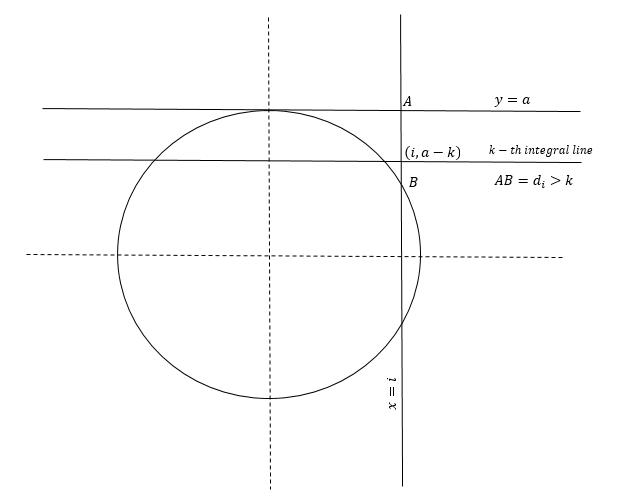
\includegraphics[width=0.5\textwidth]{diag2}
\end{figure}
\\\\ Let $(i,a-k)$ be any point on $k^{th}$ integral line, $y=a-k$. Then clearly the point $(i, a-k)$ lies within the circle if, $d_{i} \leq k$. (i.e., $a- \sqrt{a^{2}-i^{2}} \leq k$ ). Refer figure $(1)$ and $(2)$.

\begin{figure}[h]
\caption{It shows lattice point lies within circle if $d_{i}<k$.}
\centering
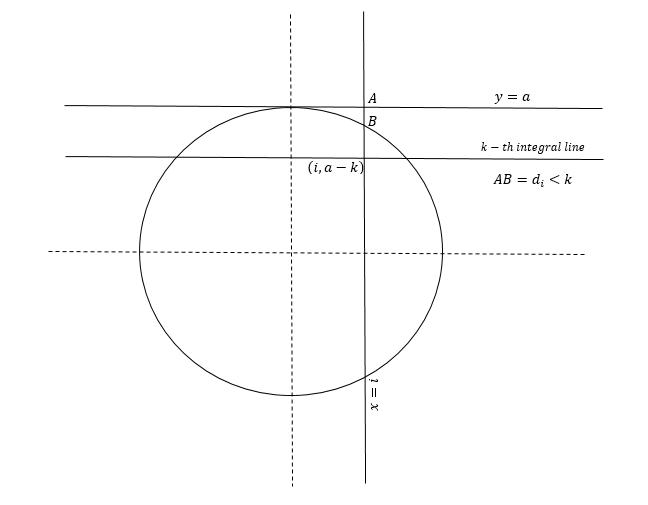
\includegraphics[width=0.5\textwidth]{diag1}
\end{figure}
Let $i_{k}$ be the maximum value of $i, i \in Z^{+}$ that satisfies the inequality $a- \sqrt{a^{2}-i^{2}} \leq k$, then all the lattice points $(i,a-k), i \in Z^{+}, i \leq i_{k}$ lie within the circle. Hence $i_{k}$ number of lattice points lie on the $k^{th}$ integral line and the section of the circle within the first quadrant. And the points are $(1,a-k), (2,a-k),......, (i_{k},a-k)$. If we include the lattice point on $k^{th}$ integral line lying on y-axis, then one more point $(0,a-k)$ is added and hence the number becomes $(i_{k}+1)$.
\\\\Let $i_{1},i_{2},i_{3},.....,i_{a}$ be the maximum integers ($i$) that satisfy inequality $a- \sqrt{a^{2}-i^{2}} \leq k, k=1,2,3,.....,a$ respectively. Then the $1^{st},2^{nd},.....,a^{th}$ integral lines contain $(i_{1}+1),(i_{2}+1),(i_{3}+1),.....,(i_{a}+1)$ points within the circle and in the first quadrant including axes. Since $a \in Z$ , the point $(0,a)$ itself is a lattice point satisfying the condition of Gauss Circle problem but does not lie on any integral line. Hence if $S$ be the total number of lattice points in the first quadrant (including axes) and within the circle then,$$ S=1+ \sum_{k=1}^{a} (i_{k}+1)$$.
\\Since, $a\in Z,$ both positive $x-$axis and positive $y-$axis include $'a'$ number of lattice points excluding origin. Hence the number of lattice points in first quadrant (excluding axes) and within the circle is, $N= (S-2a-1)$.
\\\\So, if $N(a)$ be the total number of lattice points within the circle $x^{2}+y^{2}=a^{2}$, $a \geq 0$ then,
$N(a)=4(S-2a-1)+4a+1 = 4((S-1)-a)+1$.
Hence, $$N(a)=4\bigg\{\sum_{k=1}^{a}(i_{k}+1)-a\bigg\}+1$$.
\subsection{Case 2: $a \notin Z$}
Then we replace $a$ by $[a]$ and the reference line will be $y=[a]$, where $[a]$ is the largest integer that is less than or equal to $a$. In case $(1),$ reference line contained only one lattice point, while in case $(2)$ more than one lattice point may exist. So we need to add a correction factor.
\\\\
Let $y=[a]$ and the circle intersect at point, $(h,[a]),h \in R$ in first quadrant. Then $[h]$ number of lattice point lie on the reference line intercepted in first quadrant (excluding axes). So, from the symmetry of the circle, $4[h]$ lattice points are added.
\\\\Hence, first choosing reference line as $y=[a],$ we evaluate the number of lattice points within the circle using steps in case $(1).$ Let $n(a)$ be the total lattice points obtained by the result. Then we evaluate $[h].$ Hence actual lattice points $N(a)$ can be evaluated using, $$N(a)=n(a)+4[h].$$



\section{Illustration}
Let the equation of circle be $x^{2}+y^{2}=3^{2}$,
\\Since the radius of circle$(a)$ is 3, it contain 3 integral lines. For first integral line, $k=1$, and let $i_{1}$ be the maximum integer that satisfy inequality $a- \sqrt{a^{2}-i^{2}} \leq k$. Then, $3- \sqrt{3^{2}-i_{1}^{2}} \leq 1 \Rightarrow i_{1}^{2} \leq 5 $. The maximum integer that satisfy the given inequality is 2. So, $i_{1}=2$.
\\Also, for second integral line, $k=2$, and let $i_{2}$ be the maximum integer that satisfy inequality $a- \sqrt{a^{2}-i^{2}} \leq k$. Then, $3- \sqrt{3^{2}-i_{2}^{2}} \leq 2 \Rightarrow i_{2}^{2} \leq 8 $. The maximum integer that satisfy the given inequality is 2. So, $i_{2}=2$.
\\Also, for third integral line, $k=3$, and let $i_{3}$ be the maximum integer that satisfy inequality $a- \sqrt{a^{2}-i^{3}} \leq 3$. Then, $3- \sqrt{3^{2}-i_{3}^{2}} \leq 3 \Rightarrow i_{3}^{2} \leq 9 $. The maximum integer that satisfy the given inequality is 3. So, $i_{3}=3$.
\\\\Now using, $$N(a)=4\bigg\{\sum_{k=1}^{a}(i_{k}+1)-3\bigg\}+1$$
$$N(3)=4\bigg\{\sum_{k=1}^{3}(i_{k}+1)-a\bigg\}+1$$
$$N(2)=4(i_{1}+1+i_{2}+1+i_{3}+1-3)+1= 29.$$
Hence for the circle of equation $x^{2}+y^{2}=3^{2}$, $29$ ordered pairs $(m,n)$ exist, such that $m,n \in Z$ and $m^{2}+n^{2} \leq 3^{2}$.

\section{Advancement}
The problem seems to be simple while its solution is tedious for the higher values of radius.
So why, many mathematicians have tried to relate the number of lattice points in a circle with its area. If $R$ is the radius of the circle and $N(R)$ be the number of lattice points in the circle then we write, $N(R) = \pi R^{2} + E(R)$, where $E(R)$ is some error term. 
\\Gauss managed to prove that $|E(R)| \leq 2\sqrt{2}\pi r.$

\section{Application}
It is a problem from the field of pure mathematics. This problem is important because it gives an idea of representing any integer as a sum of two squares. 
\\The results of this problem are applicable in the field of harmonic analysis, basic lattice point analysis and uncertainty principle. [3] 




\begin{thebibliography}{9}

\bibitem{IEEEhowto:kopka}
D.~Hilbert and S.Cohn-Vossen, \emph{Geometry and the imagination}, \hskip 1em plus
  0.5em minus 0.4em\relax New york: Chelsea, 1999, pp.37-38
\bibitem{IEEEhowto:kopka}
R.K~Guy, \emph{Unsolved problems in number theory},Third edition \hskip 1em plus
  0.5em minus 0.4em\relax Springer,2004, pp.365-366
\bibitem{IEEEhowto:kopka}
J.~Cilleruello, \emph{The distribution of Lattice Points on circles},\hskip 1em plus
  0.5em minus 0.4em\relax J.Number Th. 43, 1993, pp.198-202

\bibitem{IEEEhowto:kopka}
G.H.~Hardy, \emph{On the expression of a number as the sum of two squares},\hskip 1em plus
  0.5em minus 0.4em\relax Quart.J.math. 46,1915,pp. 263-283
\bibitem{IEEEhowto:kopka}
F.~Chamizo, \emph{Lattice point counting and harmonic analysis},\hskip 1em plus
  0.5em minus 0.4em\relax Madrid,2007, pp.1-18
\end{thebibliography}
%\enlargethispage{-5in}

\begin{IEEEbiography}[{
\includegraphics[width=1in,height=1.25in,clip,keepaspectratio]{hk}}]{Hemanta Kunwar}
did his Bachelors of Electrical Engineering form Pulchowk Campus, IOE, Pulchowk, Lalitpur. He has been actively participating in doing research in the field of Mathematics. His prime interest includes the use of mathematical analysis in Engineering.
\end{IEEEbiography}


\end{document}


